\documentclass[11pt]{article}
\usepackage[utf8]{inputenc}	% Para caracteres en español
\usepackage{amsmath,amsthm,amsfonts,amssymb,amscd}
\usepackage{multirow,booktabs}
\usepackage[table]{xcolor}
\usepackage{fullpage}
\usepackage[fontset=ubuntu]{ctex}
\usepackage{graphicx}
\usepackage{float}
\usepackage{subfigure}
\usepackage{lastpage}
\usepackage{enumitem}
\usepackage{fancyhdr}
\usepackage{mathrsfs}
\usepackage{wrapfig}
\usepackage{setspace}
\usepackage{calc}
\usepackage{multicol}
\usepackage{cancel}
\usepackage[retainorgcmds]{IEEEtrantools}
\usepackage[margin=3cm]{geometry}
\usepackage{amsmath}
\newlength{\tabcont}
\setlength{\parindent}{0.0in}
\setlength{\parskip}{0.05in}
\usepackage{empheq}
\usepackage{framed}
\usepackage[most]{tcolorbox}
\usepackage{xcolor}
\usepackage{mdframed}
\usepackage{soul}
\usepackage[margins,adjustmargins]{trackchanges}
\usepackage{tikz,mathpazo}
\usetikzlibrary{shapes.geometric, arrows,decorations.pathreplacing,decorations.markings,calc,arrows.meta,bending}
\usepackage{flowchart}

\tikzstyle{startstop} = [rectangle,rounded corners, minimum width=3cm,minimum height=1cm,text centered, draw=black,fill=red!30]
\tikzstyle{io} = [trapezium, trapezium left angle = 70,trapezium right angle=110,minimum width=3cm,minimum height=1cm,text centered,draw=black,fill=blue!30]
\tikzstyle{process} = [rectangle,minimum width=1cm,minimum height=0.5cm,text centered,text width =3cm,draw=black,fill=orange!30]
\tikzstyle{decision} = [rectangle,maximum width=1cm,maximum height=0.5cm,text centered,draw=black,fill=green!30]
\tikzstyle{arrow} = [thick,->,>=stealth]

\usepackage{mathpazo}
\usepackage{tkz-fct}

\usepackage{listings}
\lstset{
    language=MATLAB,
    basicstyle=\ttfamily\small,
    aboveskip={1.0\baselineskip},
    belowskip={1.0\baselineskip},
    columns=fixed,
    extendedchars=true,
    breaklines=true,
    tabsize=4,
    prebreak=\raisebox{0ex}[0ex][0ex]{\ensuremath{\hookleftarrow}},
    frame=lines,
    showtabs=false,
    showspaces=false,
    showstringspaces=false,
    keywordstyle=\color[rgb]{0.627,0.126,0.941},
    commentstyle=\color[rgb]{0.133,0.545,0.133},
    stringstyle=\color[rgb]{01,0,0},
    numbers=left,
    numberstyle=\small,
    stepnumber=1,
    numbersep=10pt,
    captionpos=t,
    escapeinside={\%*}{*)}
}

\colorlet{shadecolor}{orange!15}
\parindent 0in
\parskip 12pt
\geometry{margin=1in, headsep=0.25in}
\theoremstyle{definition}
\newtheorem{defn}{Definition}
\newtheorem{reg}{Rule}
\newtheorem{exer}{Exercise}
% \newtheorem{note}{Numerical Method Lecture Note}
\begin{document}
\setcounter{section}{0} % set counter begin from 0
\newcommand*{\num}{pi}
 % define the plot style and the axis style
\tikzset{elegant/.style={smooth,thick,samples=50,cyan}}
\tikzset{eaxis/.style={->,>=stealth}}

\title{Chapter 1 Review Notes}
%\thispagestyle{empty}

% PS: 
% {shaded} 
% is for comment 
% \begin{shaded}
% \textbf{Test}
% hello world \LeTeX
% \end{shaded}
% {mdframed}[backgroundcolor=blue!20]
% is for definition and theorem
% \begin{mdframed}[backgroundcolor=blue!20]
% test
% \end{mdframed}

%%% First You need fill out the lecture title, lecture ID and
\begin{center}
{\LARGE \bf Lecture Note Template}\\
{\large Course ID: XXX}\\
Spring 2020 \\ \\
{\large \bf Lecturer:} Prof.YOU-KNOW-WHO \ \  {\large \bfWritten by:} YOUR-NAME
\end{center}
\section{SECTION ONE}
\subsection{SUBSECTION ONE}

\textbf{Basic Idea:} Using $\LaTeX$ to write lecture note.

\begin{mdframed}[backgroundcolor=blue!20]
\textbf{Theorem One:} Just mark down the importance, not every words/sentences.
\end{mdframed}


Here is the \hl{MATLAB} code:
\begin{lstlisting}
%Program 1.1 Bisection Method
function xc=bisect(f,a,b,tol)
if sign(f(a))*sign(f(b)) >= 0
    error(’f(a)f(b)<0 not satisfied!’) %ceases execution end
    fa=f(a);
    fb=f(b);
    while (b-a)/2>tol
        c=(a+b)/2;
        fc=f(c);
        if fc == 0 %c is a solution, done
            break
        end
        if sign(fc)*sign(fa)<0 %a and c make the new interval b=c;fb=fc;
        else %c and b make the new interval
            a=c;fa=fc;
    end
end
xc=(a+b)/2; %new midpoint is best estimate
\end{lstlisting}
\begin{shaded}
For exmaple: 如何在 Overleaf 中使用中文?
\begin{itemize}
    \item[第一步:] 记得加上 ctex 这个包
    \item[第二步:] 在 Menu 里 pdfLaTeX 改成 XeLaTeX 即可
\end{itemize}
\end{shaded}
如图:
\begin{figure}[H]
    \centering
    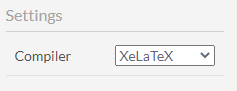
\includegraphics{Capture.PNG}
    \caption{范例图片-Sample Figure}
    \label{fig:sam-fig-1-0}
\end{figure}
多张图:
\begin{figure}[H]
\centering
\subfigure[sample-figure-one]{
    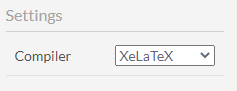
\includegraphics{Capture.PNG}
    \label{fig:sam-fig-1-1}
    }
\subfigure[sample-figure-two]{
    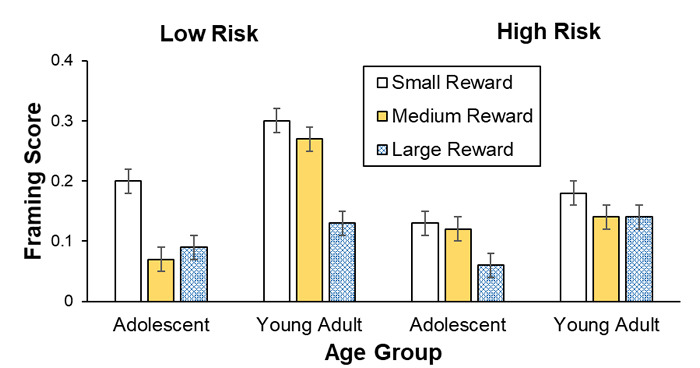
\includegraphics{sample-figure.jpg}
    \label{fig:sam-fig-2}
    }
\caption{范例图片-Sample Figure-2}
\end{figure}

我们能看到,在上面的橙色框框,似乎有东西突出来了,修改一下缩进即可:
\begin{shaded}
\textbf{如何引用 label}
\begin{itemize}[leftmargin = 100pt]
    % leftmargin 左边
    % rightmargin 右边
    % itemsep 条目之间
    \item[第一步:] 上面的图例,我们都有给他们加上标签,直接 ref 就好
    \item[第二步:] 就像这样 figure: \ \ref{fig:sam-fig-1-1}
\end{itemize}
\end{shaded}
公式范例:(三种常用的方式 align, equation 和 $\$$)
\begin{align*} % * 号的主要作用就是看后面需不需要对公式标号
    A^2 + B^2 &= C^2 \\
    C &= M^E \pmod{N}
\end{align*}
\begin{equation}
    x = \frac{-b \pm \sqrt{\Delta}}{2a}
\end{equation}
The PDF of Normal Distribution is: $P(X) = \frac{1}{\sigma\sqrt{2\pi}} exp \left[-\frac{(x - \mu)^2}{2 \sigma^2}\right]$
\end{document}

